%%%%%%%%%%%%%%%%%%%%%%%%%%%%%%%%%%%%%%%%%
% Short Sectioned Assignment LaTeX Template Version 1.0 (5/5/12)
% This template has been downloaded from: http://www.LaTeXTemplates.com
% Original author:  Frits Wenneker (http://www.howtotex.com)
% License: CC BY-NC-SA 3.0 (http://creativecommons.org/licenses/by-nc-sa/3.0/)
%%%%%%%%%%%%%%%%%%%%%%%%%%%%%%%%%%%%%%%%%

%----------------------------------------------------------------------------------------
%	PACKAGES AND OTHER DOCUMENT CONFIGURATIONS
%----------------------------------------------------------------------------------------

\documentclass[paper=a4, fontsize=11pt]{scrartcl} % A4 paper and 11pt font size

% ---- Entrada y salida de texto -----

\usepackage[T1]{fontenc} % Use 8-bit encoding that has 256 glyphs
\usepackage[utf8]{inputenc}
%\usepackage{fourier} % Use the Adobe Utopia font for the document - comment this line to return to the LaTeX default

% ---- Idioma --------

\usepackage[spanish, es-tabla]{babel} % Selecciona el español para palabras introducidas automáticamente, p.ej. "septiembre" en la fecha y especifica que se use la palabra Tabla en vez de Cuadro

% ---- Otros paquetes ----
\usepackage{alltt}
\usepackage{hyperref}
\usepackage{url} % ,href} %para incluir URLs e hipervínculos dentro del texto (aunque hay que instalar href)
\usepackage{amsmath,amsfonts,amsthm} % Math packages
%\usepackage{graphics,graphicx, floatrow} %para incluir imágenes y notas en las imágenes
\usepackage{graphics,graphicx, float} %para incluir imágenes y colocarlas

\usepackage{cite}
\usepackage{listings}
\usepackage{xcolor}

% Para hacer tablas comlejas
%\usepackage{multirow}
%\usepackage{threeparttable}

%\usepackage{sectsty} % Allows customizing section commands
%\allsectionsfont{\centering \normalfont\scshape} % Make all sections centered, the default font and small caps

\usepackage{fancyhdr} % Custom headers and footers

\setcounter{secnumdepth}{0}
\pagestyle{fancyplain} % Makes all pages in the document conform to the custom headers and footers
\fancyhead{} % No page header - if you want one, create it in the same way as the footers below
\fancyfoot[L]{} % Empty left footer
\fancyfoot[C]{} % Empty center footer
\fancyfoot[R]{\thepage} % Page numbering for right footer
\renewcommand{\headrulewidth}{0pt} % Remove header underlines
\renewcommand{\footrulewidth}{0pt} % Remove footer underlines
\setlength{\headheight}{13.6pt} % Customize the height of the header

\numberwithin{equation}{section} % Number equations within sections (i.e. 1.1, 1.2, 2.1, 2.2 instead of 1, 2, 3, 4)
\numberwithin{figure}{section} % Number figures within sections (i.e. 1.1, 1.2, 2.1, 2.2 instead of 1, 2, 3, 4)
\numberwithin{table}{section} % Number tables within sections (i.e. 1.1, 1.2, 2.1, 2.2 instead of 1, 2, 3, 4)

\setlength\parindent{0pt} % Removes all indentation from paragraphs - comment this line for an assignment with lots of text

\newcommand{\horrule}[1]{\rule{\linewidth}{#1}} % Create horizontal rule command with 1 argument of height


%----------------------------------------------------------------------------------------
%	TÍTULO Y DATOS DEL ALUMNO
%----------------------------------------------------------------------------------------

\title{	
\normalfont \normalsize 
\textsc{\textbf{Ingeniería de Servidores (2016-2017)} \\ Grado en Ingeniería Informática \\ Universidad de Granada} \\ [25pt] % Your university, school and/or department name(s)
\horrule{0.5pt} \\[0.4cm] % Thin top horizontal rule
\huge Memoria Práctica 5 \\ % The assignment title
\horrule{2pt} \\[0.5cm] % Thick bottom horizontal rule
}

\author{José Álvaro Garrido López} % Nombre y apellidos

\date{\normalsize\today} % Incluye la fecha actual

%----------------------------------------------------------------------------------------
% DOCUMENTO
%----------------------------------------------------------------------------------------

\begin{document}
\maketitle % Muestra el Títuolo

\newpage %inserta un salto de página

\tableofcontents % para generar el índice de contenidos

\listoffigures

\newpage

\newpage

\section{Cuestión 1. Al modificar los valores del kernel de este modo, no logramos que persistan después de reiniciar la máquina. ¿Qué archivo hay que editar para que los cambios sean permanentes?}

Como se explica en \cite{sysctl}, en \cite{sysctl-arch} y en \cite{sysctl-conf}, \textit{sysctl} tiene un archivo de configuración, \textit{/etc/sysctl.conf} en el que permanecen los cambios realizados sobre los parámetros del \textit{kernel} entre reinicios del sistema.
Para ello, hay que añadir o modificar las líneas correspondientes en el fichero de configuración.

Editamos el fichero \textit{/etc/sysctl.conf} como se muestra en \ref{00}, añadimos la siguiente línea al fichero, de forma que el número máximo de PIDs del \textit{kernel} sea de 65536 (el valor por defecto es de 32768):

\begin{verbatim}
kernel.pid_max = 65536
\end{verbatim}

\begin{figure}[H]
	\centering
	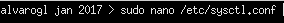
\includegraphics[scale=0.6]{00.png}
	\caption{Edición del fichero \textit{/etc/sysctl.conf}} \label{00}
\end{figure}

\begin{figure}[H]
	\centering
	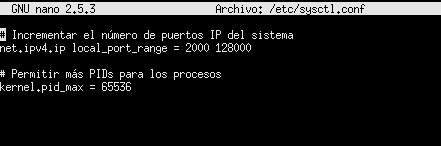
\includegraphics[scale=0.6]{01.png}
	\caption{Adición de una línea para modificar el número de PIDs de los procesos} \label{01}
\end{figure}

A continuación, en \ref{02} se muestra el parámetro modificado. Después de un reinicio, esta opción permanecerá activa.

\begin{figure}[H]
	\centering
	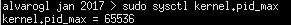
\includegraphics[scale=0.6]{02.png}
	\caption{Comprobación del nuevo valor del parámetro modificado} \label{02}
\end{figure}

\section{Cuestión 2. ¿Con qué opción se muestran todos los parámetros modificables en tiempo de ejecución? Elija dos parámetros y explique, en dos líneas, qué función tienen.}

Con la opción \textit{sysctl -a} podemos mostrar todos los parámetros del \textit{kernel} disponibles para modificar. Véase \ref{03}.

\begin{figure}[H]
	\centering
	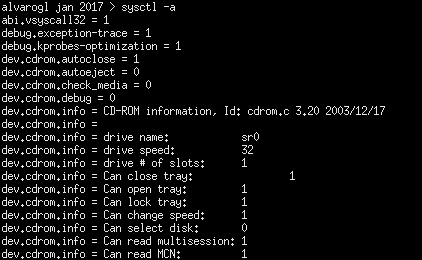
\includegraphics[scale=0.6]{03.png}
	\caption{Fragmento de la salida de \textit{sysctl -a}} \label{03}
\end{figure}

He escogido los parámetros \textit{net.ipv4.ip\_forward} y \textit{vm.swappiness}.

\begin{itemize}
\item{net.ipv4.ip\_forward: Como se explica en \cite{packetforward}, es una opción para habilitar el redireccionamiento de puertos. Esta opción viene deshabilitada por defecto, pero en caso de que la necesitemos activar porque utilizamos una VPN o por otro motivo, podemos hacerlo desde \textit{sysctl}.}
\item{vm.swappiness: En \cite{swap} se explica que es un valor entre 0 y 100 que indica el porcentaje máximo de intercambio de memoria realizable. Un valor alto mejora el rendimiento del sistema, sin embargo, para cargas de trabajo dedicadas a operaciones con bases de datos, se recomienda un valor de \textit{vm.swappiness} bajo, como 10}
\end{itemize}

\section{Cuestión 3}

\subsection{a) Realice una copia de seguridad del registro y restáurela, ilustre el proceso con capturas}

Para ello consulté la referencia \cite{backupreg}.

En primer lugar, debemos abrir el \textbf{Editor del Registro} de \textbf{Windows}. Para ello, ejecutamos regedit (acceso directo a Ejecutar: Windows + R). Véase en \ref{04}.

\begin{figure}[H]
	\centering
	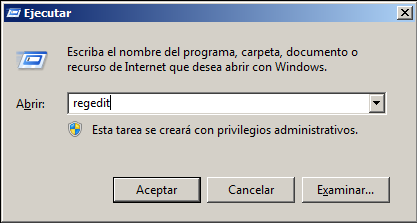
\includegraphics[scale=0.6]{04.png}
	\caption{Ejecución de \textit{regedit}} \label{04}
\end{figure}

Seleccionamos el registro del cual deseamos crear la copia de seguridad como se ve en \ref{05}.

\begin{figure}[H]
	\centering
	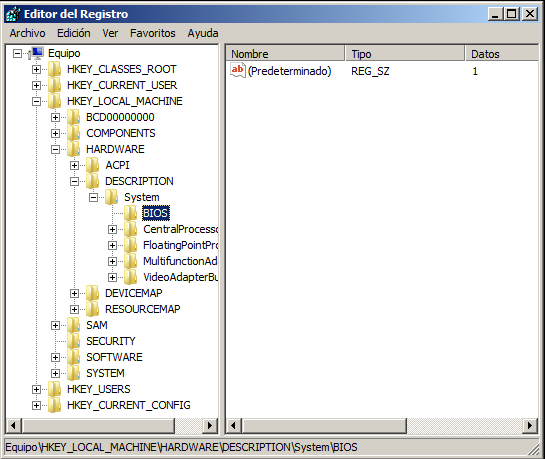
\includegraphics[scale=0.6]{05.png}
	\caption{Selección del registro de BIOS} \label{05}
\end{figure}

Nos creará un archivo con el nombre que indiquemos como aparece en \ref{06}.

\begin{figure}[H]
	\centering
	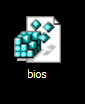
\includegraphics[scale=0.6]{06.png}
	\caption{Archivo exportado con la copia de seguridad del registro} \label{06}
\end{figure}

Una vez realizada la copia de seguridad, debemos abrir de nuevo el \textbf{Editor del Registro} y seleccionar la opción \textit{Importar archivo del Registro} del menú \textit{Archivo} de la interfaz, tal y como se muestra en \ref{07}.

\begin{figure}[H]
	\centering
	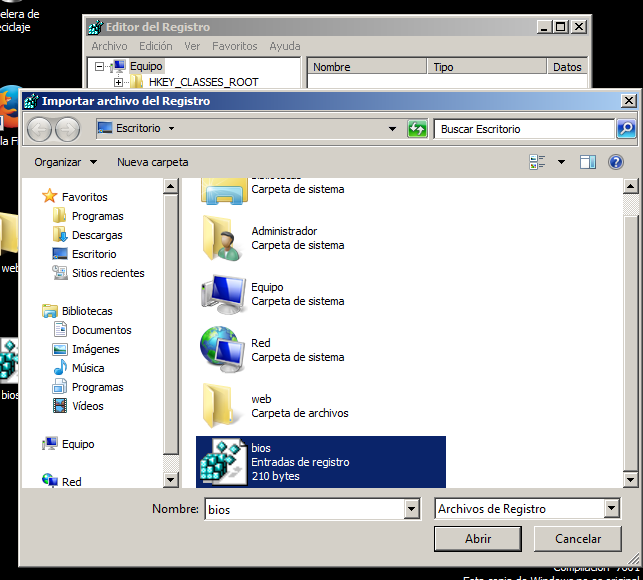
\includegraphics[scale=0.6]{07.png}
	\caption{Importación del archivo \textit{bios}} \label{07}
\end{figure}

Si todo ha ido bien, se nos mostrará la ventana que aparece en \ref{08} indicando que la restauración se ha completado con éxito.

\begin{figure}[H]
	\centering
	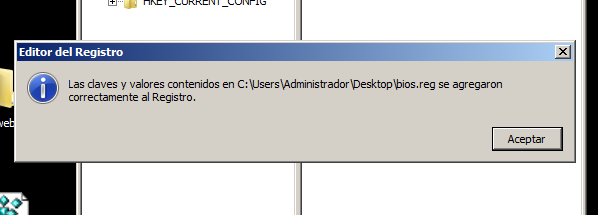
\includegraphics[scale=0.6]{08.png}
	\caption{Restauración de las claves de registro con éxito} \label{08}
\end{figure}

\subsection{b) Abra una ventana mostrando el editor del registro}

En \ref{09} se muestra la ventana del \textbf{Editor del Registro}.

\begin{figure}[H]
	\centering
	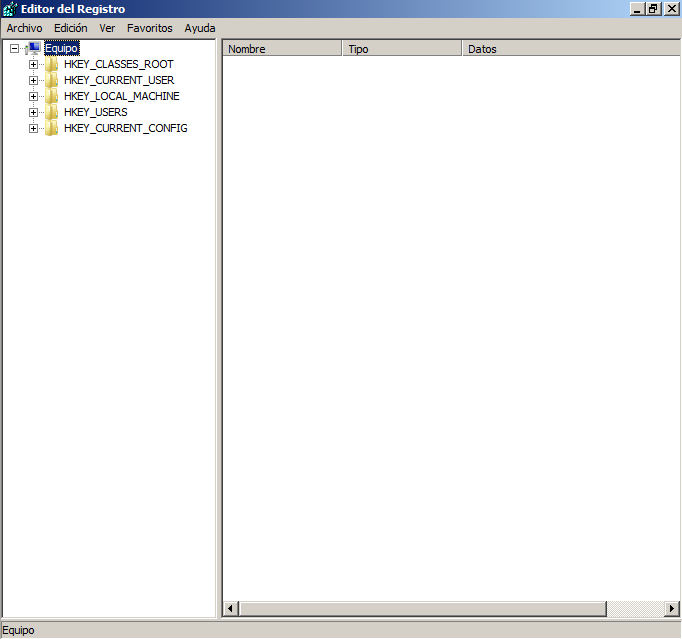
\includegraphics[scale=0.45]{09}
	\caption{Ventana de \textbf{Editor del Registro} de \textbf{Windows}} \label{09}
\end{figure}

\section{Cuestión 4. Enumere qué elementos se pueden configurar en Apache y en IIS para que Moodle funcione mejor.}

Como se explica en \cite{moodleperf}, si configuramos bien Moodle, este puede ser utilizado tanto para pocos usuarios como para cientos de ellos. Es conveniente intentar potenciar aquellos servicios que mayor demanda tengan, como por ejemplo, el rendimiento del servidor web si los usuarios pasan mayor tiempo navegando la web que consultando la base de datos.

\textbf{Configuraciones para Apache}

\begin{itemize}
\item{Cambiar la directiva MaxClients. Esta variable indica el uso de memoria máxima de los procesos de \textbf{Apache}. Por defecto, \textbf{Apache} utiliza 10 MB por proceso. Se puede cambiar este valor a 100.
Se recomienda utilizar la fórmula MaxClients = Memoria total disponible * 80 \%}
\item{Reducir el número de módulos que \textbf{Apache} carga en \textit{httpd.conf} a 20-30}
\item{Actualizar a la última versión de \textbf{Apache}}
\item{Reducir el número máximo de peticiones por hijo (\textit{MaxRequestPerChild}) a 20-30.}
\item{En caso de que la carga del servidor sea alta apagar el servicio \textit{KeepAlive}}
\item{Reducir \textit{timeout} a 30-60}
\item{Activar almacenamiento en caché}

\end{itemize}

\textbf{Configuraciones para IIS}

\begin{itemize}
\item{Los cambios se deben realizar en el archivo \textit{HKLM \textbackslash SYSTEM \textbackslash CurrentControlSet \textbackslash Services \textbackslash Inetinfo \textbackslash Parameters \textbackslash}}
\item{Cambiar \textit{ListenBackLog} a valores de 2 a 5}
\item{Modificar valor de \textit{MemCacheSize} para ajustar la cantidad de memoria que \textbf{IIS} utilizará para los archivos en caché dependiendo de las necesidades}
\item{Cambiar \textit{MaxCachedFileSize} para modificar el tamaño máximo de un archivo en caché}
\item{Crear un \textbf{DWORD} (ObjectCacheTTL) para cambiar el tiempo que un objeto puede estar en caché}

\end{itemize}

\section{Cuestión 5. Ajuste la compresión en el servidor y analice su comportamiento usando varios valores para el tamaño de archivo a partir del cual comprimir. Para comprobar que está comprimiendo puede usar el navegador o comandos como curl (see url) o lynx. Muestre capturas de pantalla de todo el proceso.}

Seguimos las guías de \cite{configcompr} y de \cite{curl}.
Inicialmente, sin compresión, el archivo ocupa 316750 B, como se muestra en \ref{12}

\begin{figure}[H]
	\centering
	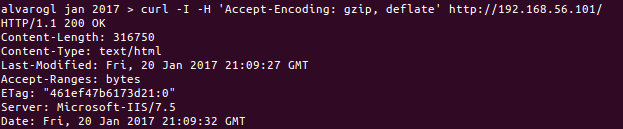
\includegraphics[scale=0.6]{12.png}
	\caption{\textit{curl}, resultado sin compresión inicial} \label{12}
\end{figure}

Si habilitamos la compresión a partir de tamaño 2700 B de archivo, como se muestra en \ref{14}, conseguimos una reducción importante en el tamaño.

\begin{figure}[H]
	\centering
	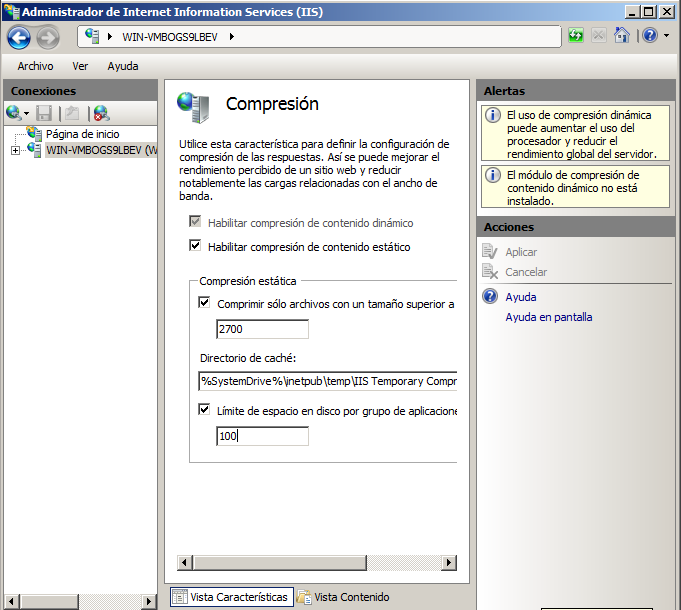
\includegraphics[scale=0.45]{14.png}
	\caption{Habilitación de la compresión (1) } \label{14}
\end{figure}

Como se ve en \ref{13}, ahora el tamaño del archivo es de 120301 B y el contenido está comprimido (gzip).

\begin{figure}[H]
	\centering
	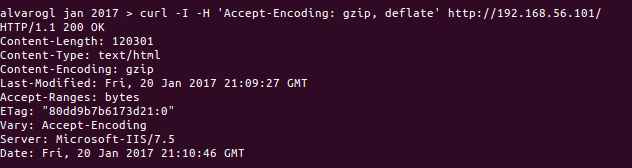
\includegraphics[scale=0.6]{13.png}
	\caption{\textit{curl}, resultado con compresión} \label{13}
\end{figure}

Cambiamos ahora el tamaño mínimo para comprimir a 400000 B de tamaño de archivo, de manera que nuestro archivo de 316750 B no se comprimiría. Ver \ref{15}.

\begin{figure}[H]
	\centering
	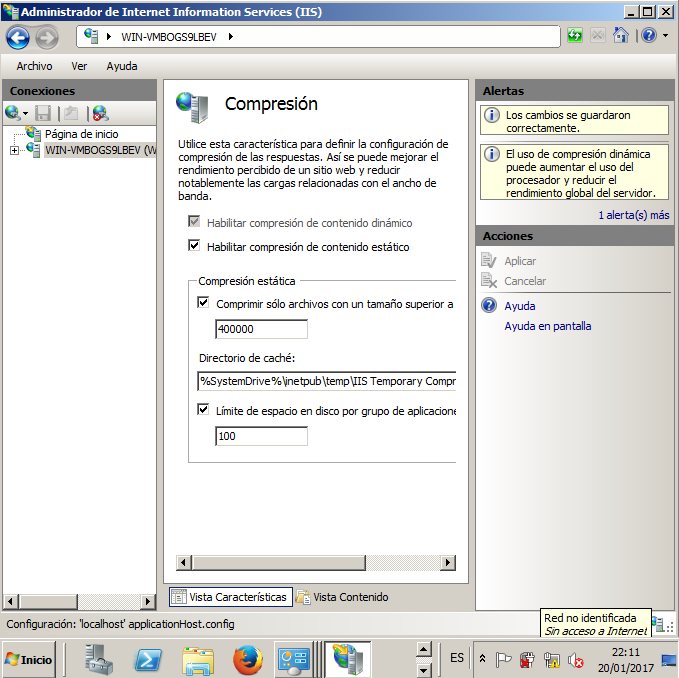
\includegraphics[scale=0.45]{15.png}
	\caption{Habilitación de la compresión (2) } \label{15}
\end{figure}

En \ref{16} se observa que tras habilitar la compresión para tamaños de archivo mayores que el nuestro, no se comprime.

\begin{figure}[H]
	\centering
	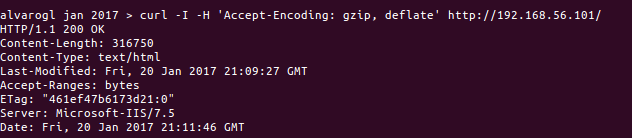
\includegraphics[scale=0.6]{16.png}
	\caption{\textit{curl}, resultado sin compresión por tamaño de archivo inferior al configurado} \label{16}
\end{figure}

\section{Cuestión 6. Usted parte de un SO con ciertos parámetros definidos en la instalación (Práctica 1), ya sabe instalar servicios (Práctica 2) y cómo monitorizarlos (Práctica 3) cuando los somete a cargas (Práctica 4).} 

\subsection{a) Al igual que ha visto cómo se puede mejorar un servidor web (Práctica 5 Sección 3.1), elija un servicio (el que usted quiera) y modifique un parámetro para mejorar su comportamiento.}

En mi caso he escogido configurar \textbf{Apache} para obtener un mayor rendimiento a la hora de servir las peticiones. Para medir el rendimiento utilizaremos \textbf{Apache Benchmark (ab)}.

Entre las opciones que se explican en \cite{apache-doc}, se habla de \textit{HostnameLookups}, una directiva que habilita la búsqueda de DNS en las direcciones IP del cliente, lo cual puede producir un poco de retardo.

\subsection{b) Monitorice el servicio antes y después de la modificación del parámetro aplicando cargas al sistema (antes y después) mostrando los resultados de la monitorización.}

Si desactivamos esta opción como se observa en \ref{18}, conseguiremos un mejor rendimiento, y al realizar una prueba con 400000 peticiones, el tiempo reducido al atenderlas disminuirá considerablemente.

En \ref{17} se observa el resultado del \textit{benchmark} con la opción activa (unos 138 segundos), y en \ref{19}, el resultado con la opción desactivada (unos 118 segundos). Con la opción inhabilitada ha sido 20 segundos más rápido el proceso.

\begin{figure}[H]
	\centering
	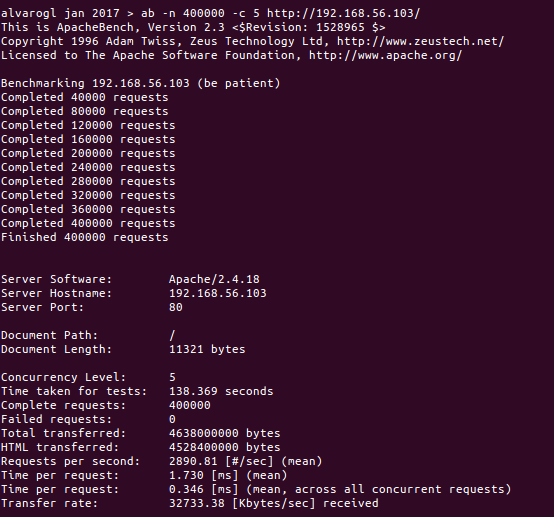
\includegraphics[scale=0.6]{17.png}
	\caption{\textit{Apache benchmark} con la opción \textit{HostnameLookups} activada} \label{17}
\end{figure}

\begin{figure}[H]
	\centering
	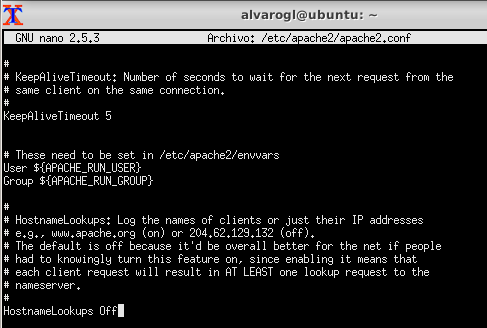
\includegraphics[scale=0.6]{18.png}
	\caption{Edición del fichero \textit{/etc/apache2/apache2.conf}} \label{18}
\end{figure}

\begin{figure}[H]
	\centering
	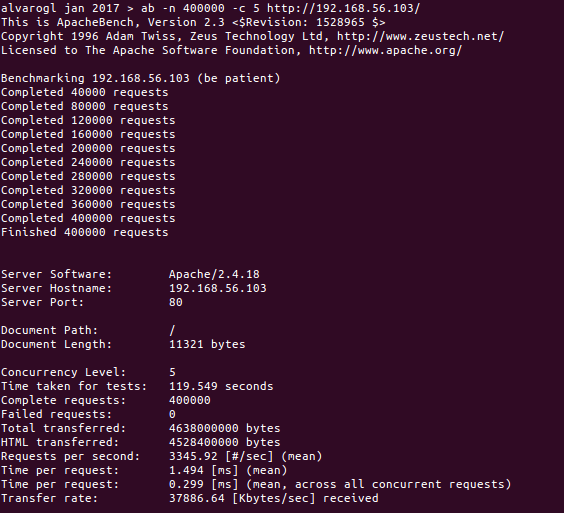
\includegraphics[scale=0.6]{19.png}
	\caption{\textit{Apache benchmark} con la opción \textit{HostnameLookups} desactivada} \label{19}
\end{figure}

\newpage
\bibliographystyle{plain}
\bibliography{biblio}

\end{document}